\documentclass[]{acm_proc_article-sp}
\usepackage{graphicx}
\usepackage{listings}
\usepackage{float}
\usepackage{color}
\usepackage{courier}
\usepackage[usenames,dvipsnames]{xcolor}
\usepackage{enumitem}

\newcommand{\commentout}[1]{}
\newcommand{\todo}[1]{\textbf{[TODO: #1]}}
% To disable, just uncomment this line 
% \renewcommand{\todo}[1]{\relax}
\renewcommand{\thefootnote}{\fnsymbol{footnote}}

\begin{document}

\title{Resource Based Assignment of Queries in Distributed Databases}

\numberofauthors{3}
\author{
%\alignauthor
  David Dietrich, Tzu-Yang Yu, Yiyao Liu \\
  David R. Cheriton School of Computer Science \\
  University of Waterloo \\
  Waterloo, Canada \\
  \email{\{d4dietri, t32yu, y435liu\}@uwaterloo.ca}
}

\maketitle

%To fix up those stupid underfull hbox warnings
% http://tex.stackexchange.com/questions/138/what-are-underfull-hboxes-and-vboxes-and-how-can-i-get-rid-of-them

\begin{abstract}
Distributed database is blablabla. However, a disadvantage of such database is the imbalanced workload assigned to each node server and thus the inefficiency of the whole system. In this paper, we examine how the different CPU and memory usage on a machine affect the query execution time.  Based on that, we try to assign jobs to different node servers according to their conditions. From our experiment, 
\end{abstract}

\section{Introduction}

Recently, the cloud has attracted a lot of attention from both the scientific research community and practitioners as it enables executing long running resource intensive tasks on the cloud using as many nodes as required thus greatly reducing the task completion time and eliminating the need to procure expensive server grade hardware~\cite{Agrawal:2008:CRD:1462571.1462573}. However, the performance of cloud compute nodes is often not consistent, with some nodes obtaining orders of magnitude worse performance than other nodes. There are a variety of reasons a node could suffer from degraded performance, ranging from extremely heavy workload (i.e., the node is a hotspot), to partial hardware failure~\cite{citeulike:6656195}. However, the modern scheduling systems only simply assigned query to the closest replica~\cite{borthakur-07}, without taking heterogeneous hardware into account. This eventually limits communication between servers, and making congestion and computation hot-spots prevalent even when spare capacity is available elsewhere.

In this paper we describe Horoscope, a resource based query assignment algorithm for distributed databases. The goal of our work is to explore an efficient way to schedule queries based on server conditions, such as resource usage, hardware condition and network traffic in order to attain better performance and alleviate hotspots. We first start by using CPU and memory usage information to scheduling queries; however, due to time and environmental constraints, we have not explored the possibility of using other related resource usage. The contributions of our paper are the following. First, we implement our scheduling algorithm on the Apache Cassandra~\cite{ Lakshman:2010:CDS:1773912.1773922} open source distributed file project. Second, we implement an algorithm for assigning queries to nodes based upon the CPU and Memory (RAM) usage of the nodes. Third, we ran a series experiments and found that our algorithm provides a benefit under certain circumstances. Finally, we found that other factors that we feel are very important (e.g., disk seek time, distance between servers, and network traffic) for our implementation. We take those factors into consideration and further develop a new formula that we believe would more closely resemble the resource requirements for executing a query.
 
The remainder of this paper is organized as follow. In Section~\ref{sec:relWork}, we describe several areas related work.

\section{Related Work}
\label{sec:relWork}

To work around this problem, many researchers focus on estimating workload resource usage in order to maximal performance while minimizing the cost of resources used~\cite{citeulike:6656217,5452742,curino2011relational, MIT-Relational}. This predict job execution time and resource requirements technique can help cloud provider to make decision about which requests from which users are to be executed on which computational resources, and when~\cite{citeulike:6656217}. Many researchers had built workload placement recommendation service base on workload demand patterns~\cite{Gmach:2007:WAD:1524302.1524818, Atikoglu:2012:WAL:2254756.2254766}, and such approach can result in 35\% reduction in processor usage~\cite{Gmach:2007:WAD:1524302.1524818}. Differ to our study, our system do not take workload requirement perdition into account, because we believe that execute workload analysis for every query will result in some latency issues. Instead, our system focuses on dynamically forwarding workload to the idlest server, in order to prevent hotspot.
 
Furthermore, some other researchers focus on partitioning schemes. Works like graph partitioning algorithms~\cite{Karypis:1998:FHQ:305219.305248}, workload-aware partitioning~\cite{Scholl:2009:WDP:1516360.1516366}, and classical work on physical design and partitioning~\cite{Zilio:1998:PDD:928651} are focusing on dividing data into partitions that maximize transaction/query performance to allow workloads to scale across multiple computing nodes. However, graph partitioning is NP-hard problems, and solutions to this problem are generally derived using heuristics and approximation algorithms~\cite{citeulike:11192678}, and we believe that this will introduce execution complexity, and the performance is vary to different databases. Next, the workload-aware partitioning focus on partition tables base on workload prediction~\cite{Scholl:2009:WDP:1516360.1516366, Mit-Shinobi}; however, there are many workloads, a finite number can be hosted by each server, and each workload has capacity requirements that may frequently change based on business needs~\cite{Gmach:2007:WAD:1524302.1524818}, this means that workload-aware partitioning needs to be dynamic rather than static; however dynamic workload-aware partitioning will reduce performance dramatically. Last, some other works on physical design and partitioning allows database loaded into the system by both static decision and dynamic decision in order to increase I/O bandwidth~\cite{Zilio:1998:PDD:928651}. This approach is pragmatic, but if we only rely on partitioning database the performance will be limited.
 
Virtual machine (VM) migration is also another approach for load balancing. VM migration focuses on the transfer of a VM from one physical machine to another with little or no service downtime (e.g. live VM migration) when the server that the VM sits on becomes overloaded with processes, traffic, or memory usage~\cite{Clark:2005:LMV:1251203.1251223}. Nevertheless, the challenges with long distance live migration are the WAN bandwidth, latency, and packet loss limitations that are outside the control of most IT organizations. Many applications are susceptible to network issues across the WAN that can be exacerbated by distance and network quality~\cite{murphyVMWare}, in addition, traditional VM migration will cause network traffic and bandwidth consumption, and many VM migration researcher are struggling in mitigating those causes~\cite{Liu:2009:LMV:1551609.1551630}.


\section{Design}
\label{sec:design}

In order to better utilize the various servers in a distributed database and prevent servers from becoming hotspots, we have designed a method to assign jobs based on server conditions. A program runs on all of the servers in the cluster and periodically measures the servers' resource usage (e.g., CPU Usage). When the master server receives a query from a client it examines the resource usage of all the servers in the cluster. It chooses the server with the lowest resource usage (the one that is the most likely to finish a query fastest) to assign the query to. In this way, we will hopefully mitigate hotspots on node servers, balance the workload and eventually improve the overall performance of the database. In the remainder of this section, we will state our assumptions about the working environment, give a detailed description of the overall design and provide a typical example of how the program will flow.

\subsection{Assumptions}
For scoping reasons we have made several assumptions about the database:

\begin{itemize}

\item The ultimate goal for this project is to make a methodology that is generally applicable to any kind of database. However, in this project, we will only focus on distributed key-value databases.

\item We only consider database setups that have a  that have a single master server. This is done to reduce the complexity of the clusters that we consider in our design. Because a single master server handles the whole system, we focused on reducing the overhead of the master server (which will be discussed in more detail in Section~\ref{sec:implementation}).

\end{itemize}

We have created two different programs that will measure the resource usage of each node and collect the resource usage information of each node on the master server.

The program running on every node is called the Resource Monitor(RM). The RM measures the server conditions by measuring values such as the CPU and Memory (RAM) usage. After obtaining the resource usage values, a resource usage score is calculated using the following equation:

\begin{center}
$ResourceUsage = \frac{1}{1-CPU} \times \frac{1}{1-Memory}$
\end{center}

The $CPU$ value is the CPU usage of the machine as a percentage value between 0 and 1. The $Memory$ value is a ratio of the used memory divided by the total memory. The formula above has been shown in previous work to be a good indicator of the computing cability of a server~\cite{Wood:2007:BGS:1973430.1973447}.

The program running on the master server is called the Central Job Director (CJD). The CJD is responsible for collecting the resource usage scores from the RMs and determining which node should be assigned a particular query.

Figure~\ref{fig:designFig} illustrates how the communication between the RM, CJD and database occurs. The resource usage score is periodically sent from the RM to the CJD. By passively receiving the resource scores the master server can get the updated node server condition with very little overhead. If the master server were to ask for the score actively there would not only be twice as many network messages to retrieve the resource score, but there would also be the possibility of the CJD becoming blocked and waiting for a reply from a node server. The only downside of doing it this way is that the RM must be aware of the IP address of the master server. After collecting the scores, the CJD stores them and makes them available through an API to the database. The database can use these values to determine the optimal location to process a query. The exact method of communication between the CJD and database will be discussed in more detail in Section~\ref{sec:implementation}.

\begin{figure}[t]
\centering
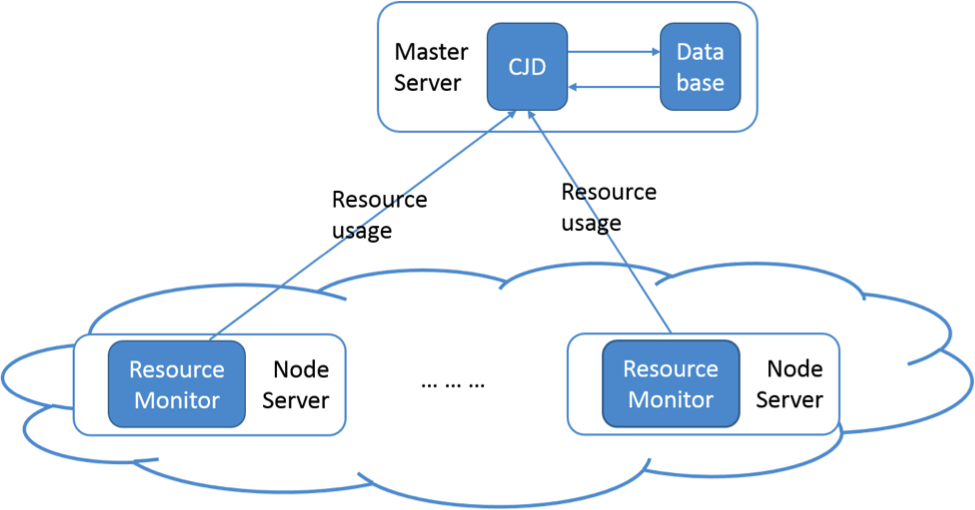
\includegraphics[scale=0.5]{images/design.png}
\caption{The physical design of a cluster using our resource usage based query assignment algorithm.}
\label{fig:designFig}
\end{figure}

\section{Implementation}
\label{sec:implementation}
In this section, we present the detailed implementation methodology for our query assignment algorithm. In the implementation used in our project we are using Apache Cassandra~\cite{ Lakshman:2010:CDS:1773912.1773922}. To scope our project, we only implemented the algorithm for single-key reads and scans. In the remainder of this section we will first present the implementations of the RM, CJD, and the modifications to Cassandra.

\subsection{The Resource Monitor}
The RM resides on each of the node servers in the cluster. To measure the CPU and Memory usage of the server we are using JavaSysMon\footnote{https://github.com/jezhumble/javasysmon}. Every 1 second the RM sends a UDP packet containing its resource usage score to the CJD server. We chose a 1 second interval because we do not feel that the increased information gained by a smaller interval is enough to justify the increased overhead on the network and server processing ability. In addition, given the relatively short amount of time it takes to process a query (even scans) we do not believe it is possible for the RM to send packets fast enough that the algorithm can its assignment decision based on the execution of a single query. For these reasons we are more interested in determining if a node is being consistently heavily loaded, so that we can assign queries to other nodes in the cluster.

\subsection{The Central Job Director}
The CJD runs as a separate program on the master server and is responsible for collecting resource scores of all node servers, storing the data and making that data available to the database. It listens to the network and receives all of the UDP packets from the RMs. Each packet provides the node address and resource usage value for that node. This information is then stored in a hash table. To make the resource usage information available to the database we are using Java's Remote Method Invocation~\cite{JavaRMI}. The database can then call the remote method (this is straightforward with Cassandra as it is written in Java) and retrieve the hash table containing the node addresses and their resource usages.

\subsection{Cassandra}
We have chosen to diverge from our original design and implement the assignment logic within Cassandra instead of the CJD (to reduce the number of inter-process calls). We modified the Cassandra code that performs single-key reads to assign a query to the replica that has the lowest resource usage. The exception to this is the case where a replica is already located on the master server, at which point we always assign the query to the master (to avoid needing the additional network communication). This part of code is extremely critical because it runs every time the database receives a read query. If it is slow, the performance of the database will be bad no matter how accurate the resource usage score is. We will discuss how we reduced the overhead in Section~\ref{sec:impl_overhead}.

The assignment logic for scans is similar to the logic for reads, but it also considers that the range of keys may exist on several different replicas.

We should note that the CJD could have been implemented within Cassandra (as they both exist on the same server). However, we chose to keep them separate to reduce the coupling of our method to Cassandra and make things easier to move around on the cluster.

\subsection{Reducing overhead}
\label{sec:impl_overhead}

With a single master server directing all queries it is critical that the performance of the query assigner remains high. Also, too much overhead at master server will affect the scalability of the database. Therefore, we took several steps to reduce the overhead at the master server:

\begin{itemize}
\item
For sending information between the RM and the CJD, UDP is used instead of TCP.

\item
To reduce the number of inter-process calls Cassandra also maintains a hash table that stores the resource usage scores for the server. This table is updated once per second when the resource usage scores are updated on the CJD. We have taken steps to ensure that the hash table storing the resource usage information in Cassandra is never locked due to updates. 
\end{itemize}


\section{Evaluation}
To evaluate our scheduling algorithm we are comparing the performance of Apache Cassandra (version 1.1.6)~\cite{Lakshman:2010:CDS:1773912.1773922} with and without our scheduler. We have chosen to use Cassandra because it is an open-source key-value database with a large community and is used by several enterprise clients~\cite{DataStaxCassandra}. To evaluate the performance of each version of Cassandra we are using the Yahoo! Cloud Service Benchmark (YCSB)~\cite{Cooper:2010:BCS:1807128.1807152}. The remainder of this section will describe the experimental setup and the results of the experiments.

\subsection{Experimental Configuration}
Our experiments were performed on a 10-server cluster running Ubuntu Linux 12.04. Each server has a 6-core 2.3GHz processor and 16GB of main memory. The machines are all located in close proximity (latency did not prove to be an issue in the experiments).

The data in Cassandra was partitioned using the \textit{RandomPartitioner} (equivalent to Consistent Hash Partitioning~\cite{consistentHashPartitioning}). The data was therefore equally distributed between all 10 nodes in the cluster (the Master server contained data to be queried on, but this did not appear to result in the master being overloaded). The replication factor used in our database was three. The read consistency was set to \textit{one} (meaning that the read query only looks at a single replica to get a result).

The baseline method for assigning queries to nodes in a Cassandra cluster is the \textit{SimpleStrategy}. This method just assigns the query to the first replica in the ring. It should be noted that this method is only adequate for single data-center databases (which is the only situation we have tested). Cassandra offers other choices (e.g., a method for a database distributed over multiple data centers and for use with Amazon’s EC2 cloud environment), but given our experimental hardware configuration we did not explore these methods.

YCSB is used to generate and insert the data for the experiments. All of the data is stored in a single database table. There are 10 values associated with each key, with each value being 100 bytes. We ran our experiments on databases with 10 million keys and 150 million keys (corresponding to 10GB and 150GB databases). This was done to examine the impact that Cassandra’s key and row caching would have on the comparative performance of the versions of Cassandra.

We ran two different kinds of workloads against Cassandra: a 100\% read workload, and a 100\% scan (multi-key read) workload. The read-heavy workload was used because reads are the most time consuming single-key operation, and likewise scans are the most time consuming operation overall. The maximum scan length was set to 1000 keys, with the distribution over that range being uniform.

The queries are generated dynamically conforming to a Zipfian distribution~\cite{Gray:1994:QGB:191843.191886} with a skew of 0.99. We chose to use a Zipfian distribution so that the workload would differ between machines in the cluster (thus making our scheduling algorithm more applicable). The YCSB clients were run from one of the machines in the cluster (not the master). This did not appear to have any effect on the performance of the scheduler. 

The performance is measured in terms of operations per second that are performed. This is the default method that YCSB provides to measure performance. The YCSB also offers the ability to set a target for the number of operations that should be performed per second (similar to deadlines on the queries). However, this method sets the same deadline for every query and is directly related to the throughput, so we have chosen to only examine throughput. Each experiment has been performed using 5, 10, 20, 50 and 100 parallel YCSB clients.

\subsection{Experimental Results}
In this section, the performance with and without the scheduler is compared in each graph; the dashed line is the performance of the baseline Cassandra and the solid line is the performance using our scheduler. The Cassandra cluster was restarted between every run. The results are averaged over 3 runs each.

A problem that arose somewhat often was issues of test environment consistency between experimental runs. That is, it is not entirely uncommon for a node to crash during operation. Initially, we did not examine the node status after each run, and therefore our initial results from the experiments could be quite skewed in favor of one method or the other. In addition, one of the nodes in the cluster did not have its time synchronized with the other nodes, resulting the schema disagreement issues that caused that particular node to drastically decrease its performance. After recognizing that this was causing skewed results we re-ran all of our experiments and took these issues into account.

\begin{figure*}[t]
\centering
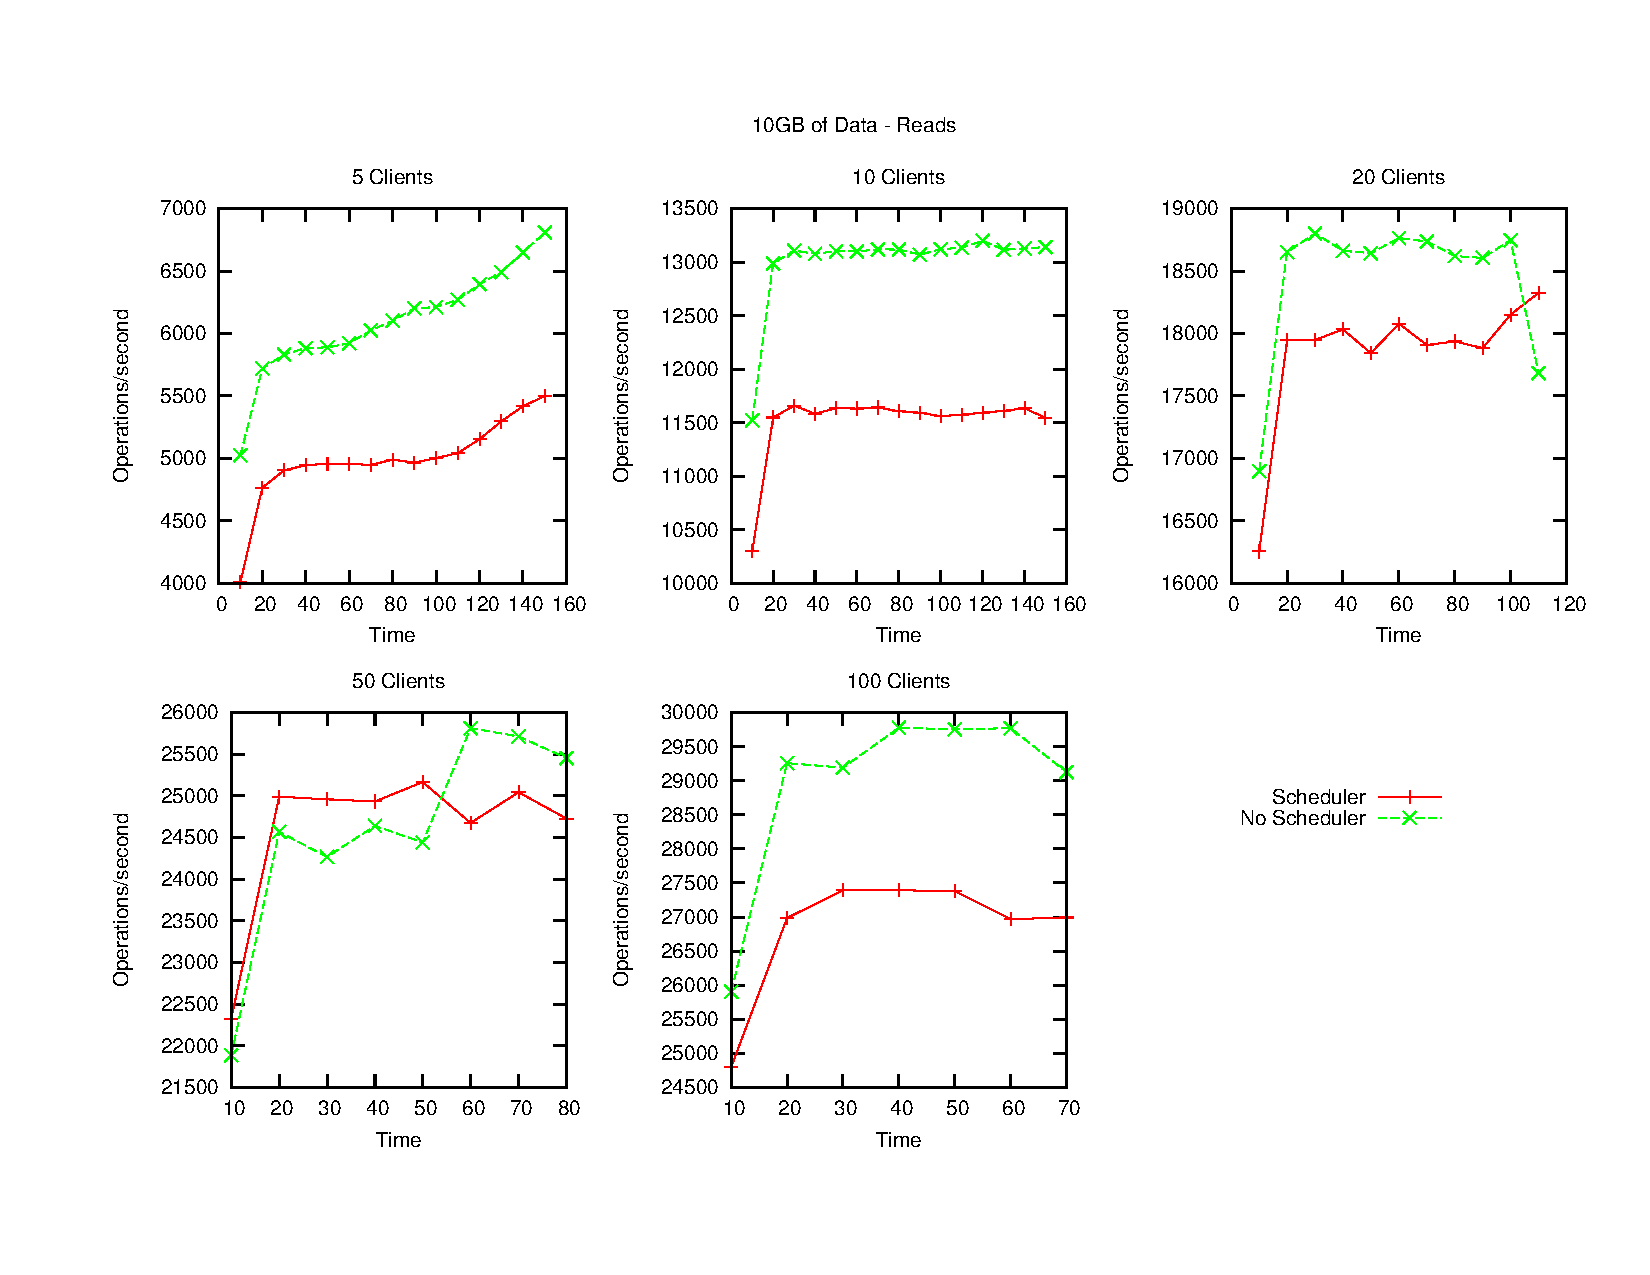
\includegraphics[scale=0.563]{images/10GB_Reads.pdf}
\vspace{-15pt}
\caption{The experimental results of performing the 100\% read workload on the 10GB database.}
\label{fig:10g_reads}
\end{figure*}

The results of the 10GB experiment are shown in Figure~\ref{fig:10g_reads}. As can be seen, the version of Cassandra using the resource based query assignment did not perform nearly as well as the baseline version. However, the difference in throughput between the scheduled and baseline versions tended to stay constant throughout the course of each experiment. As well, the ratio of the difference between experiments was very similar. This seems to indicate that the overhead of performing the additional assignment logic is what resulted in the decrease in performance. We also monitored the servers resource usage during the course of the experiment and found that the server was never heavily loaded, which means that the performance difference is very minor (i.e., there is no noticable difference between 10\% CPU usage and 12\% CPU usage).

\begin{figure*}[t]
\centering
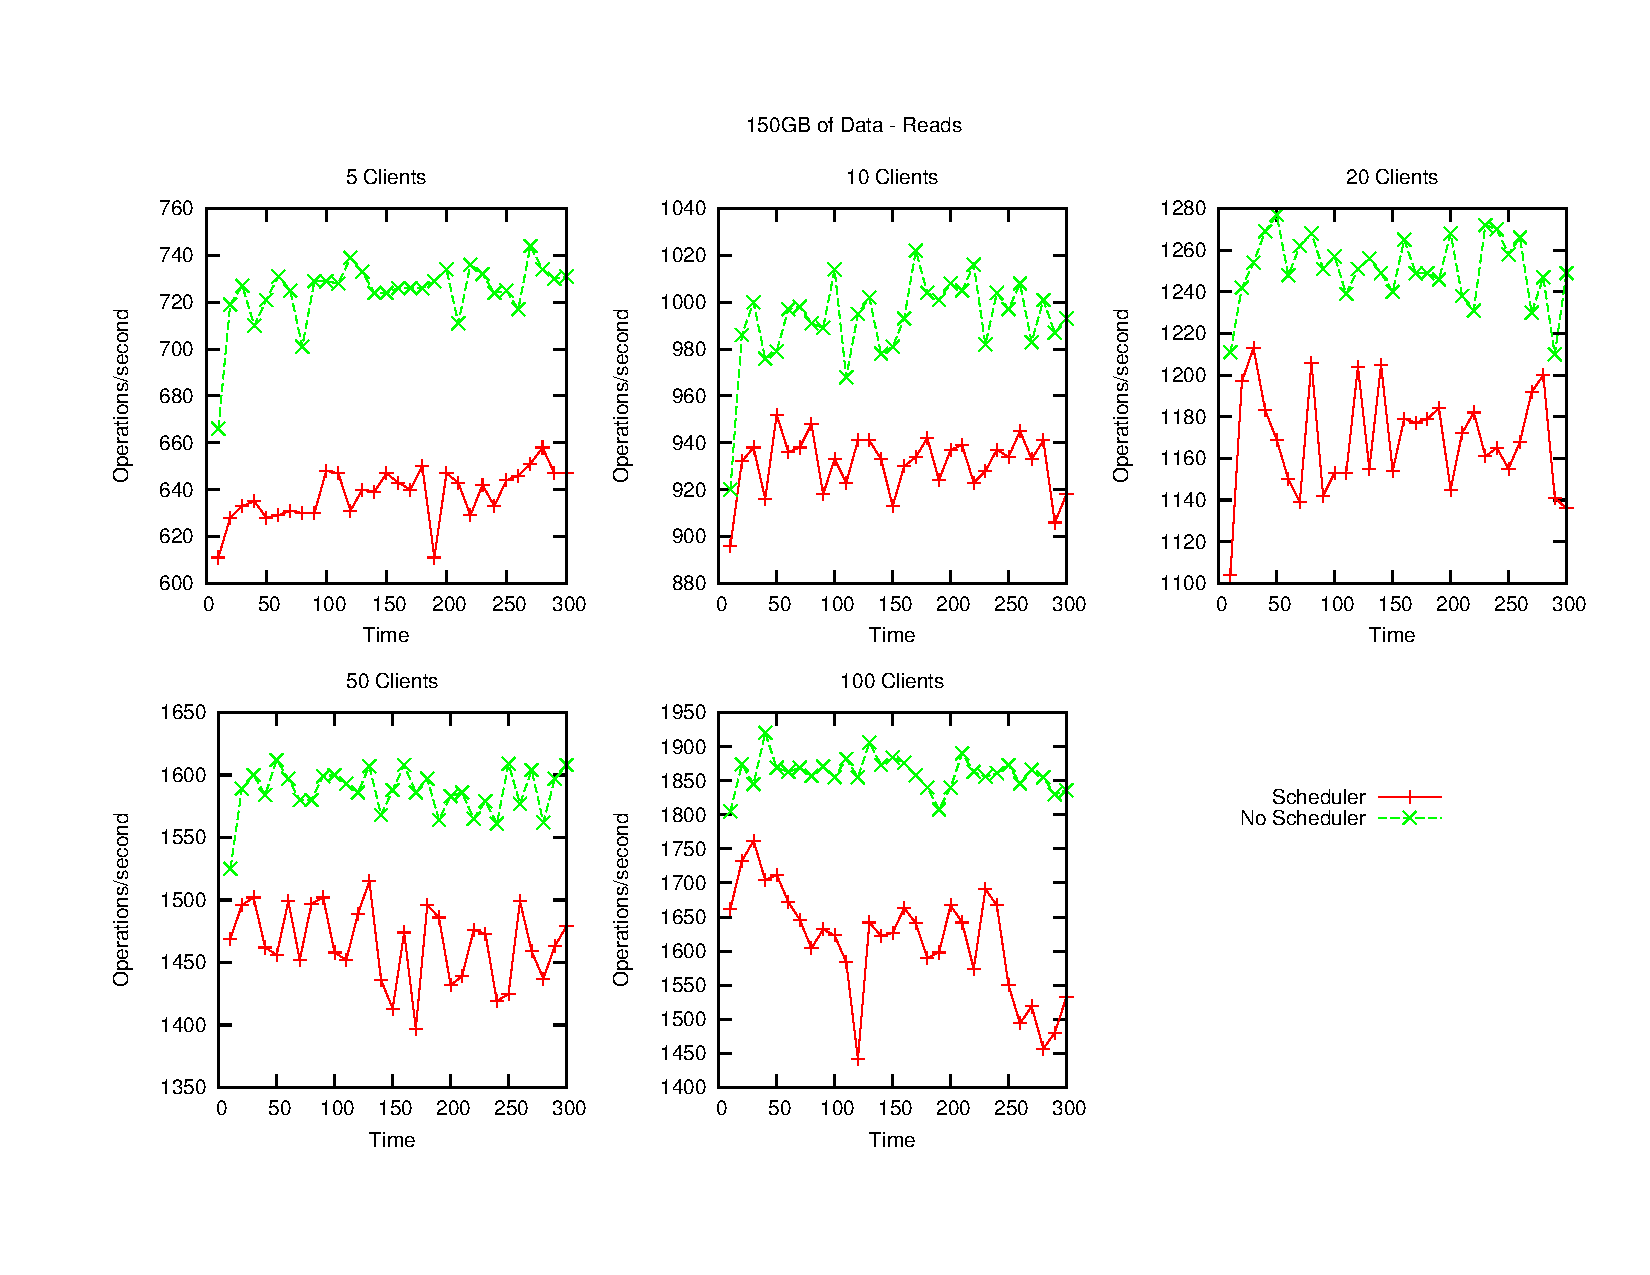
\includegraphics[scale=0.563]{images/150GB_Reads.pdf}
\vspace{-15pt}
\caption{The experimental results of performing the 100\% read workload on the 150GB database.}
\label{fig:150g_reads}
\end{figure*}

The results of running the 100\% read workload on a 150GB database are shown in Figure~\ref{fig:150g_reads}. As before, the scheduled version of Cassandra is slower than the baseline version in every case. The difference is performance is approximately 100 operations/second the 5, 10, 20 and 50 client experiments; the difference rises to over 150 operations/second in the experiment that uses 100 parallel clients.

We believe that the poor performance of the scheduling algorithm during the read workload is due to three reasons:

\begin{enumerate}

\item Even while 100 parallel clients were sending queries to the database, the node servers CPU usage and memory usage was very low. Therefore, the difference in throughput between the 150GB and 10GB databases (30000 operations/second versus 1900 operations/second) seems to indicate that hard-disk accesses are the bottleneck (this makes sense considering this is the bottleneck in traditional databases as well). This means that our resource usage formula is missing an important part of what determines how quickly a query can execute.

\item The introduced overhead of the scheduling logic seems to have a significant impact on our performance. This is especially apparent in the experiments on the 10GB database, where much of the data could be stored in the database cache. We believe that that this is what causes the throughput in the 10GB database experiments to differ by almost 1000 operations per second.

Unfortunately, this is not something that can be easily resolved. The baseline version of Cassandra does not perform any kind of analysis of the replica servers and instead just sends the query to the first replica. In our algorithm we are adding an additional thread and network calls to Cassandra, as well as scanning a vector of length $n$ (where $n$ = number of replicas) and finding the replica with the smallest resource value. In isolation these actions do not cause a noticeable drop in performance, but when performing 30000 reads per second there is significant overhead.

\item Another reason why the scheduled read could never have better performance than the unscheduled version is because of the use of read digests~\cite{readDigest} in Cassandra. A read digest is used to maintain consistency of replicas in the database. For every read query, Cassandra will read the value from the first replica, but also get a MD5 hash of the values on all of the other replicas. This is what Cassandra uses to gain eventual consistency. Naturally, a problem arises because even though we are reading the actual value from the least loaded replica, we are still querying the heavily loaded replicas to get a hash of the value.

It is for this reason that we have also examined how our assignment operation performs when applied to the scan operation (which does not perform a read digest).

\end{enumerate}

\begin{figure*}[t]
\centering
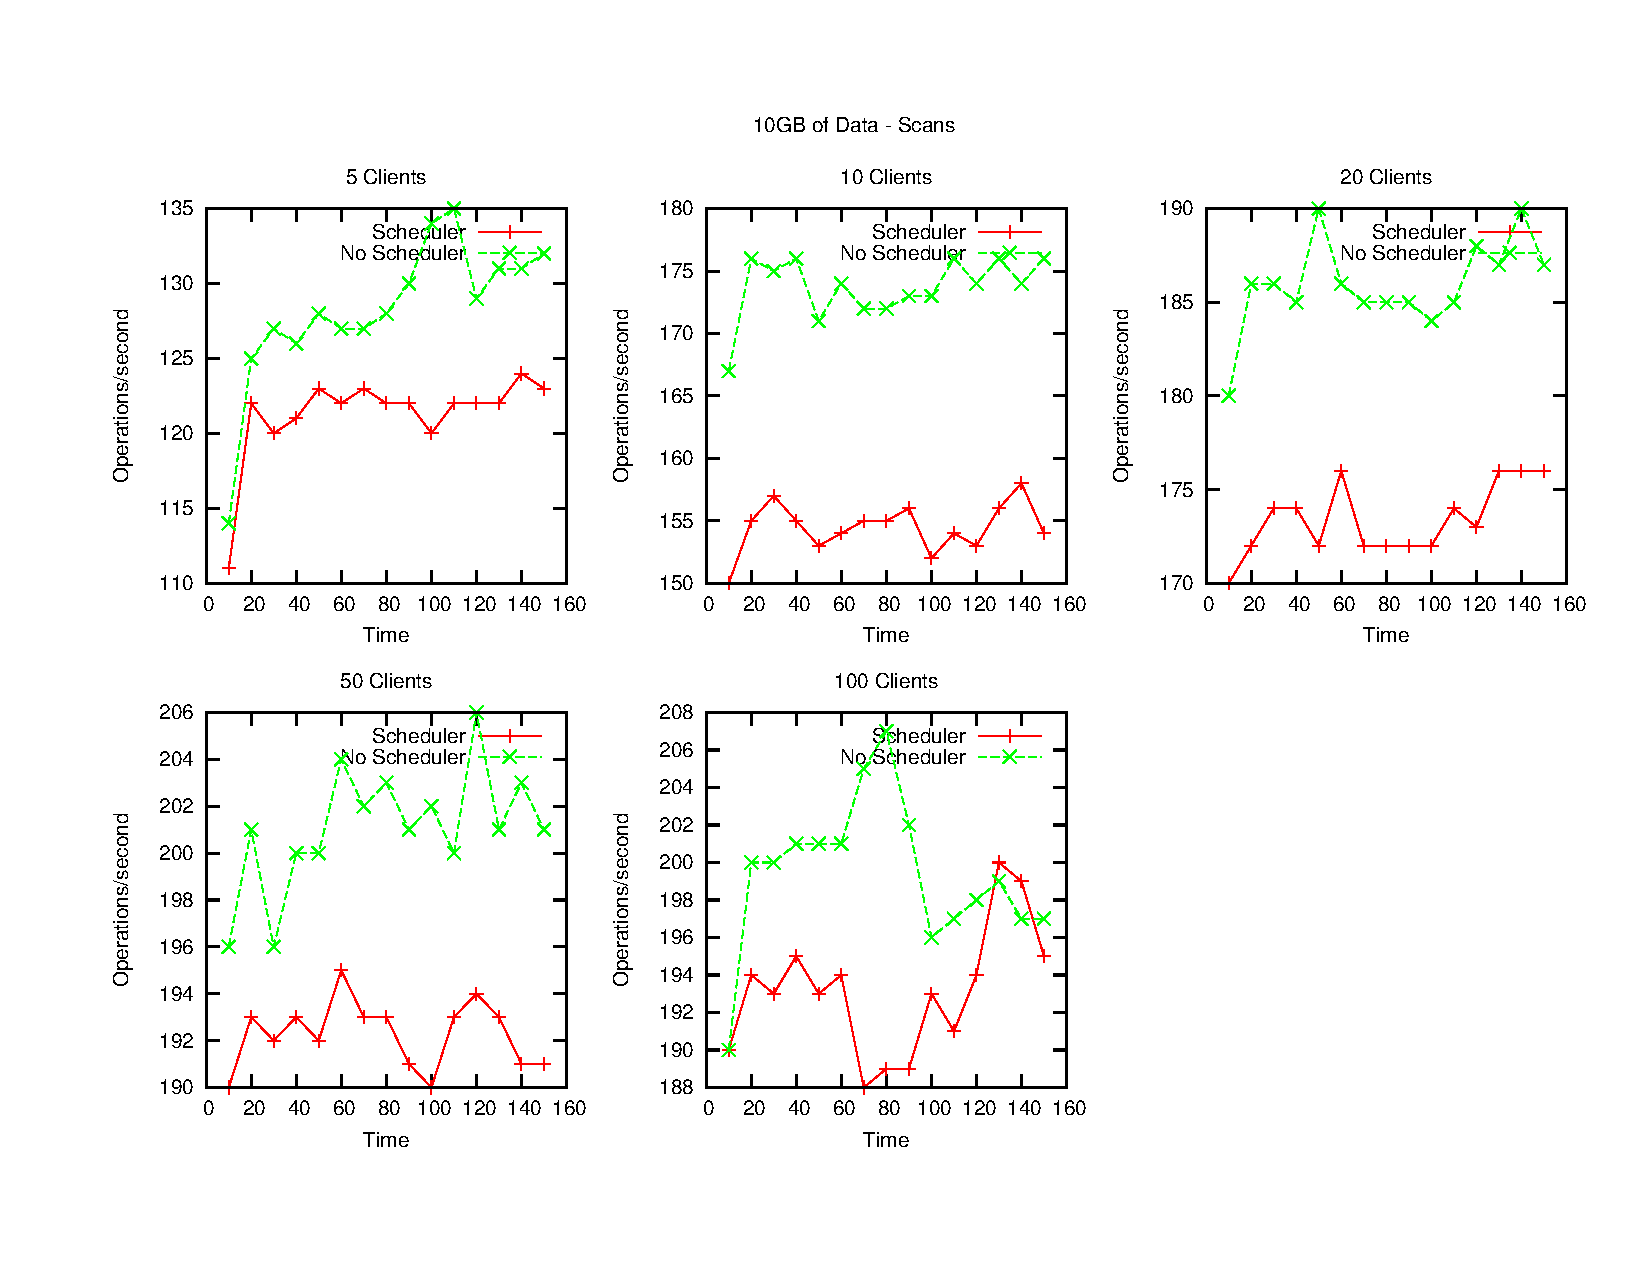
\includegraphics[scale=0.5]{images/10GB_Scans.pdf}
\vspace{-15pt}
\caption{The experimental results of performing the 100\% scan workload on the 10GB database.}
\label{fig:10g_scans}
\end{figure*}

The results of the scans experiment on the 10GB database are shown in Figure~\ref{fig:10g_scans}. In these experiments the performance of both versions of Cassandra are very close to one another. The results are particularly close for the experiments with 50 and 100 concurrent clients. We believe this is because when there are a high number of concurrent clients the CPU and memory usage varies enough between node servers that the query execution time is affected. We attempted to test with a greater number of clients than 100 (both 500 and 1000) and in both cases the results were similar because it appears that the master server became too heavily loaded.

Averaging the results of the experiments over 3 runs is not enough to say conclusively if the scheduled version of Cassandra provides better performance than the baseline version when performing scans with large numbers of concurrent clients. However, it appears that the performance of Cassandra when using the scheduling algorithm is at least on par with the performance of the baseline version of Cassandra. When the resource usage formula is improved to take factors other than CPU usage and memory usage into account it should, hopefully, provide consistently better performance than the baseline version of Cassandra. Confirming this requires further testing.

\begin{figure}[t]
\centering
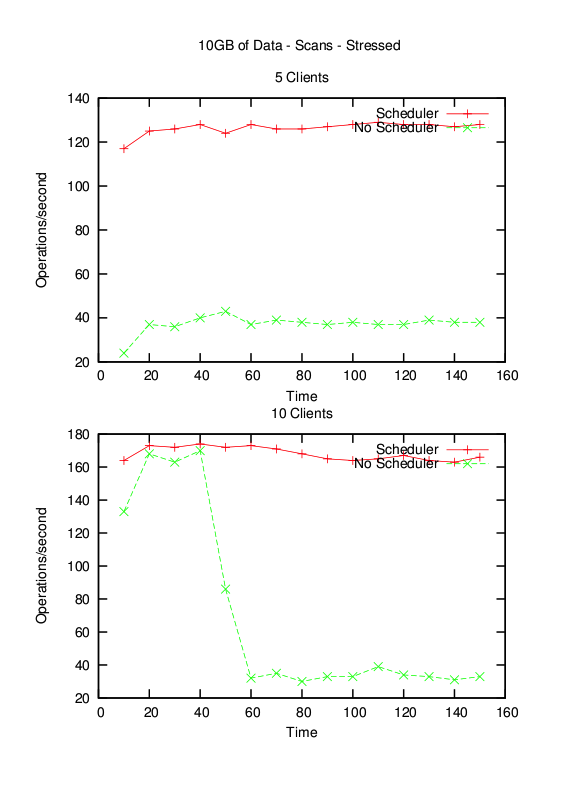
\includegraphics[scale=0.4]{images/10GB_Scans_Stressed.png}
\vspace{-15pt}
\caption{The experimental results of performing the 100\% scan workload on the 10GB database (where every second node is stressed).}
\label{fig:10g_scans_stressed}
\end{figure}

We also ran the 100\% scans workload on the 10GB database while introducing artificial CPU and memory work into the server (this was done using the stress\footnote{ http://weather.ou.edu/~apw/projects/stress/} tool). Every second node in the cluster was loaded by starting 30 processes that would continually malloc() and free() data. This resulted in fairly constant 100\% CPU and memory usage.

The results of the 5 and 10 client experiments are shown in Figure~\ref{fig:10g_scans_stressed}. In these cases you can see that the resource aware assignment has much better performance than the baseline Cassandra. This is because the resource aware assignment will consider that every second server is overloaded and not send queries to those servers. The results for the baseline version of Cassandra are taken from a single run of the YCSB. This is because the consequent runs all resulted in the YCSB throwing numerous exceptions before aborting. The figures for the cases with 20, 50 and 100 clients are not shown because performing experiments on the baseline version of Cassandra resulted in the YCSB benchmark continually aborting during the middle of the experiments. We believe this occurs because the queries sent to the heavily loaded server may be significantly delayed or lost, resulting in the YCSB believing the something is wrong with Cassandra (though we have not confirmed if this is actually the reason).

Although server load similar to the artificial load that we introduced may be quite rare in practice, we believe that this is the ideal environment to use our query assignment algorithm.

\section{Discussion}
\label{sec:discussion}

As can be seen, our approach only provides a noticeable improvement to the performance of Cassandra when multiple nodes in the cluster are heavily loaded. This is not what we initially imagined our results would be. One of our intuitions is that the performance decrease exists because the resource usage formula does not accurately reflect what the time to execute a query will be. To confirm this intuition we performed an experiment that compared the resource usage to the query execution time in a Cassandra instance.

In the remainder of this section we will provide what we feel will be a more accurate resource usage formula for distributed databases, as well as discuss several limitations that may also have affected our work.

\subsection{Re-examining the Resource Usage formula}
\label{sec:examineResUse}

\begin{figure}[t]
\centering
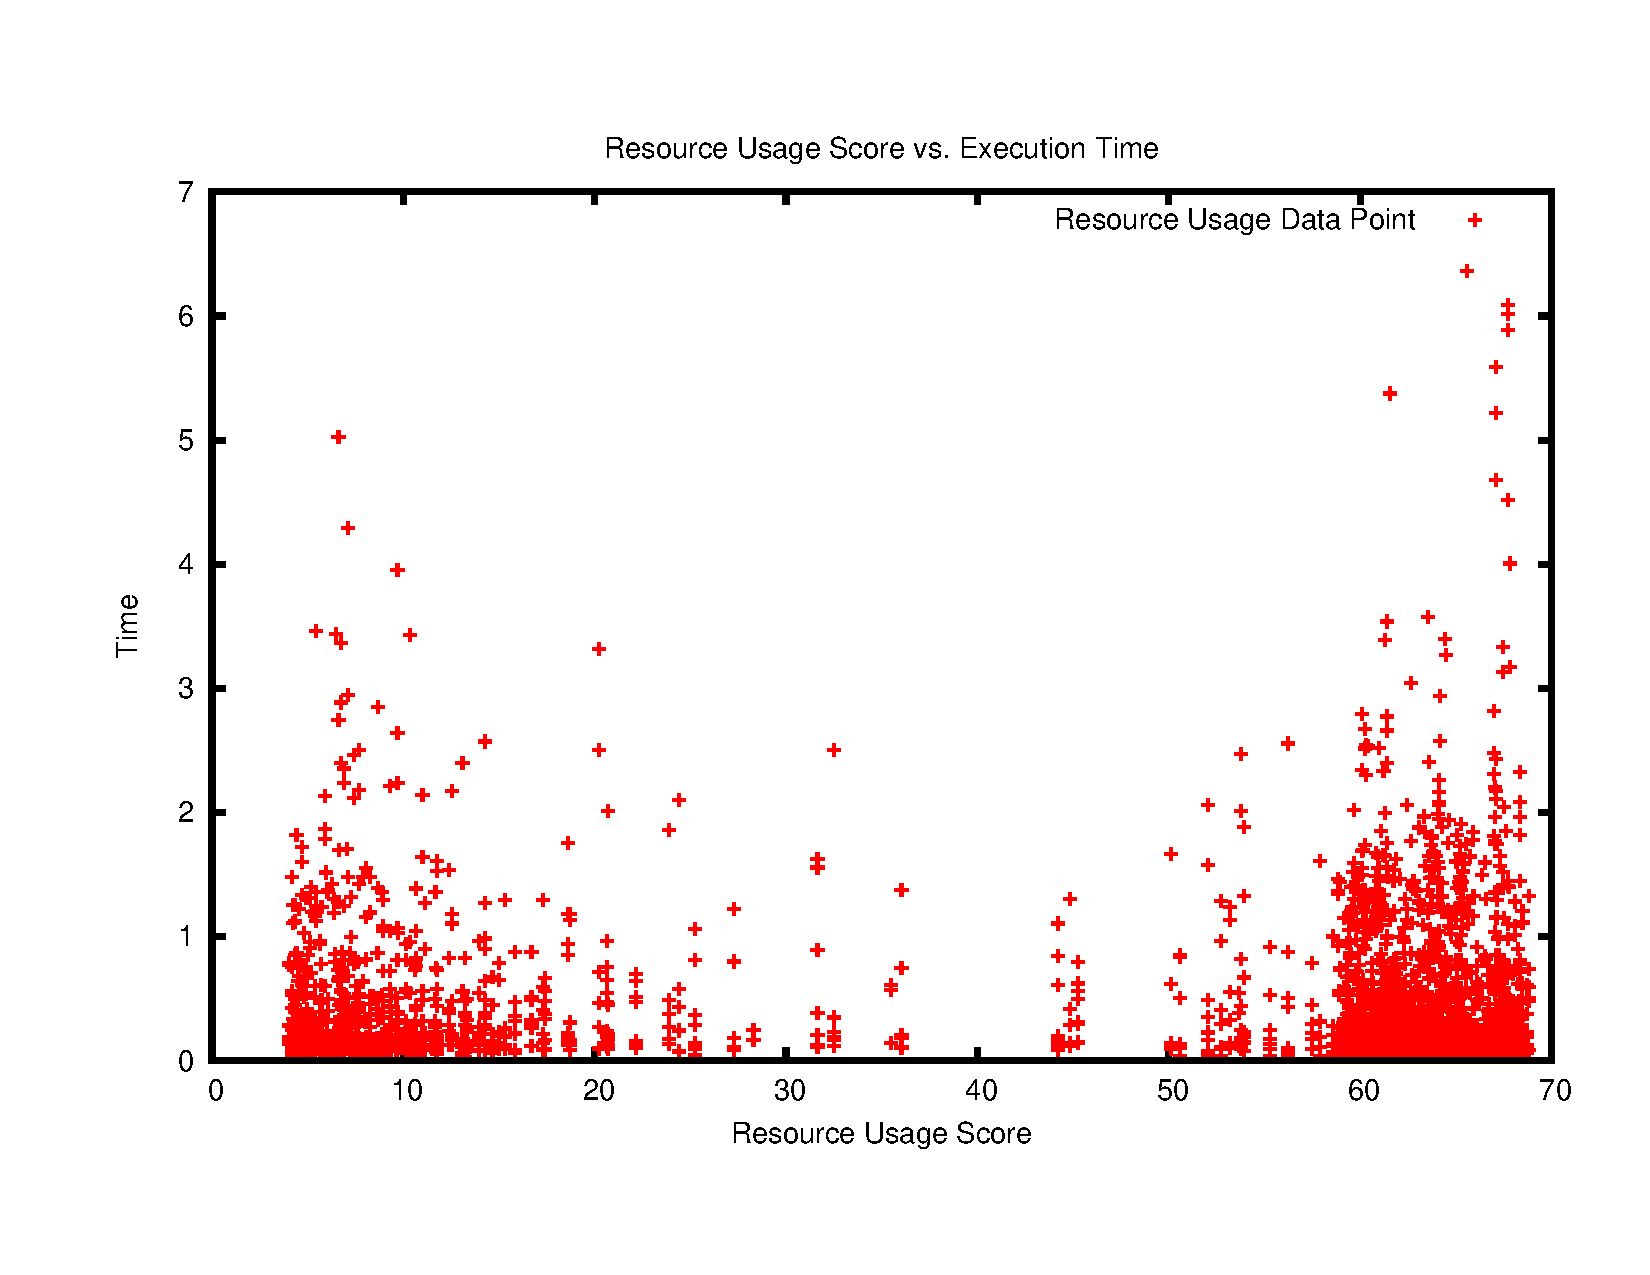
\includegraphics[scale=0.3]{images/ResUse.pdf}
\vspace{-15pt}
\caption{The experimental results comparing the resource usage score to the query execution time.}
\label{fig:resourceUsageFig}
\end{figure}

To examine how representative the resource usage score is we have performed an experiment that compares resource usage to query execution time. The setup for the resource usage experiments is different than the setup for the primary experiments. This experiment was performed on a single Cassandra instance on a single machine with a 4-core 2.6Ghz processor and 8GB of memory. The server also contained a solid-state drive instead of the hard disk drive used in the servers in the cluster. The settings for YCSB and Cassandra were identical, except that the replication factor was set to \textit{one}.

The CPU usage and memory usage was recorded every 250ms, and the query execution time was recorded for each query. The queries that executed in that 250ms window had their execution time averaged. The CPU usage and memory usage were used to calculate the resource usage of the server for each 250ms interval. The results were gathered over a 300 second interval using 10 parallel YCSB clients. Given our previous results showing that even 1000 parallel clients did not heavily load the node servers we do not believe that the results would be any different for a number of parallel clients greater than 10.

The results from the experiment are shown in Figure~\ref{fig:resourceUsageFig}. There appears to be little correlation between the resource usage score and the query execution time. When the resource usage score is higher, there are slightly more outliers that require a longer execution time, but in most cases the execution time seems to be independent of the resource usage. In addition, the resource usage scores tend to either be very low or very high. While this experiment was running, we also periodically loaded the server with other work. This resulted in a higher resource usage score, but not in a higher query execution time.

This experiment seems to indicate that the current formula is not ideal for determining the resource usage of the server. However, we believe that this could still work if the formula was changed to reflect how some variables affect the query execution time much more.  Additional variables can also be added that affect query execution time. For example, one of the primary bottlenecks in any database system is the hard disk, and we do not consider any variables related to the disk (e.g., disk access throughput).

Something to note is that the heap memory of the Cassandra instance rarely exceeded 1GB. Meaning that the memory usage score had little effect during the normal experiments. Even when the server was being artificially loaded the heap memory therefore has little effect. This also means that little data is being cached, which increases the importance of measuring the disk load.

\subsection{The New Resource Usage Formula}
\label{sec:usageFormula}
As Section~\ref{sec:examineResUse} shows, the resource usage score is far from ideal. We have some ideas on how to create a better resource usage formula. For reference, the current resource usage formula is:

\begin{center}
$ResourceUsage = \frac{1}{1-CPU} \times \frac{1}{1-Memory}$
\end{center}

The new resource usage formula is:
\begin{center}
$ResourceUsage = \frac{1}{1-CPU} \times j\left ( \frac{1}{1-Memory} \right ) \times k\left ( \frac{1}{1-Disk} \right ) \times \frac{1}{1-Distance}$
\end{center}

This is our proposed new equation that we feel may be more representative of the machine condition and should work better as a reference for assigning jobs. As can be seen, the \textit{CPU usage} and \textit{Memory usage} are still in the equation. We have added parameters for \textit{Disk} usage, \textit{Distance} (network overhead) and two scaling parameters:

\begin{itemize}
\item{\textit{Disk}} \\
\textit{Disk} refers to the hard disk performance of the machine. We feel this value should be related to values such as the average disk access time and data transfer rate. It will also be related to the disk usage condition by all programs on the machine. The slower the disk is by nature, and the busier the disk is being used by the programs, the higher the value of \textit{Disk} will be. 
\item{Distance} \\
\textit{Distance} is referring to the distance between the node servers and the network conditions. This value will be determined by both the physical network ability, like the total available bandwidth; and the network conditions, like current network usage. This parameter is very important in affecting affect the execution time when dealing with multiple datacenters.
\item{Parameters \textit{k,j}} \\
The different server performance parameters have a different magnitude of effect on the query execution time. For example, from what we observed during the experiments, memory usage has little influence on the query execution time while \textit{disk usage} affects the execution time a lot. This importance level is adjusted by the constant coefficients \textit{j} and \textit{k} in the equations. \textit{Memory} is less important so \textit{j} should probably be less than 1 and \textit{disk} is very important so \textit{k} is probably bigger than 1. The exact value of these parameters would need to be determined with further testing.
\end{itemize}

This equation is just a representation of our idea and isn't necessarily accurate. More experiments are needed to confirm that this equation leads to better performance. 

\subsection{Limitations}
Our system only provides better performance in very limited cases. Apart from the reasons listed in Section~\ref{sec:experiments} we believe that our experiment is limited due to the following reasons:

\paragraph{Limited test environment}
As mentioned earlier, we only have ten servers in our experiment which limits the replica allocation. The distance between the servers is also extremely short, such that latency was never as issue. In reality, there are an average of 100,000 servers in a data center~\cite{Guo:2010:SDC:1921168.1921188}, and replication and backup processes may occur between data centers~\cite{F5-Accelerate}. In addition, normally every one mile in distance will add 8.2 microseconds latency to the performance, and this number does not consider package drop, switch delay, and link size~\cite{Cisco-Latency}. This implies that one mile in distance between servers will have a delay greater than 8.2 microseconds. Replication between datacenters and a large amount of servers will result in longer distance communication, and this is, we believe, the distance between servers is also a very important factor while performing workload partitioning.
 
\paragraph{Simplistic workload}
The queries, which we use for testing our system, are too simple. Even though we implement our algorithm on the most time consuming queries in Cassandra the CPU and memory consumption is still rare. This is because we are using a key-value database where the operations are fairly simple and multiple optimizations have already been implemented. This seems to partially account for why our approach does not introduce any performance improvement to the original query assignment system.
 
\paragraph{Unable to congest the network manually}
Network congestion occurs when a link is carrying so much data that is greater than the capacity of the network. This causes queuing delay, packet loss, and a high chance of failure~\cite{103559}. However, we do not have this issue in our experiment, because our severs are located in close proximity and the network is never congested. This eliminates the chance to test our system under this situation.
 
\paragraph{Disk information was not considered}
Many researchers point out that the hard disk drive access times are lagging behind processor improvements, and consequently, the performance gap between processors and hard disk drives is increasing. This results in I/O wait time increasing as a percentage of processor utilization. As result, disk bottlenecks occur~\cite{IBM-IO, TMS-SSD}. This problem can partially solved by using a large amount of main memory, so as to avoid disk access for intermediate results; however main memory is not free and infinite. When there are large amount of multi-query workloads are trying to perform I/O operation, the memory will be filled up and disk bottlenecks~\cite{Bouganim:1998:MSL:288627.288646} will occur. This indicates that the disk seek time is crucial. However, our experiment only examined CPU time, which is always fast and does not have a very significant impact on the query execution time.

\subsection{Future Work}
As mentioned above, we want to validate our proposed new resource usage formula (see Section~\ref{sec:usageFormula}) by running experiments on it. After determining a more accurate representation for the resource usage of a machine, the experiments could be redone to see if it leads to better performance. At the same time, we should continue to reduce the overhead of the query assignment algorithm as overhead is one of the key factors that affect the performance of the database.

We would also like to test our new algorithm on other key-value databases (e.g., HBase) and other types of databases (e.g., distributed relational databases). In the case of relational databases, more complex queries could be used to see how the complexity of queries affect the performance.

\section{Conclusion}
\label{sec:conclusion}

Because the code that handles scans is completely disjoint from the code that handles reads, writes or updates it is plausible to implement our algorithm purely for scans while losing very little performance (just the overhead of a single thread in Cassandra that queries the CJD for resource information).


\bibliographystyle{abbrv}
\bibliography{refs}

\end{document}